% These lines can probably stay unchanged, although you can remove the last
% two packages if you're not making pictures with tikz.
\documentclass[11pt,addpoints,answers]{exam}
\RequirePackage{amssymb, amsfonts, amsmath, latexsym, verbatim, xspace, setspace}
\RequirePackage{tikz, pgflibraryplotmarks}

% By default LaTeX uses large margins.  This doesn't work well on exams; problems
% end up in the "middle" of the page, reducing the amount of space for students
% to work on them.
\usepackage{float}
\usepackage[utf8]{inputenc}
\usepackage{graphicx}
\usepackage[margin=1in]{geometry}
\usepackage[labelformat=simple,font={footnotesize}]{caption}
\usepackage{tikz}
\usepackage{circuitikz}
\usepackage{listings}
\usepackage{hyperref}
\hypersetup{
	colorlinks=true,
	linkcolor=blue,
	filecolor=magenta,      
	urlcolor=cyan,
}

% Here's where you edit the Class, Exam, Date, etc.
\newcommand{\class}{Tel-102}
\newcommand{\term}{2º Semestre 2023}
\newcommand{\examnum}{Taller}
\newcommand{\examdate}{}
%\newcommand{\timelimit}{90 Minutos}
\renewcommand{\figurename}{Figura}
\renewcommand{\solutiontitle}{\noindent\textbf{Solución:}}
\renewcommand{\theenumii}{\arabic{enumii}}
\pointname{pts}

% For an exam, single spacing is most appropriate
\singlespacing
% \onehalfspacing
% \doublespacing

% For an exam, we generally want to turn off paragraph indentation
\parindent 0ex

\lstset{
     literate=%
         {á}{{\'a}}1
         {í}{{\'i}}1
         {é}{{\'e}}1
         {ú}{{\'u}}1
         {ó}{{\'o}}1
         {¿}{{?`}}1
}

\begin{document} 

% These commands set up the running header on the top of the exam pages
\pagestyle{head}
\firstpageheader{}{}{}
\runningheader{\class}{\examnum\ - Página \thepage\ de \numpages}{\examdate}
\runningheadrule


\begin{flushright}
\begin{tabular}{p{2.8in} r l}
\textbf{\class} &  & \makebox[3in]{}\\
\textbf{\term} &&\\
\textbf{\examnum} &&\\
\textbf{\examdate} &&\\
%\textbf{Tiempo límite: \timelimit} & %\textbf{Nota:}: & \makebox[2in]{\hrulefill}
\end{tabular}\\
\end{flushright}
\rule[1ex]{\textwidth}{.1pt}

%%%%%%%%%%%%%%%%%%%%%%%%%%%%%%%%%%%%%%%%%%%%%%%%%%%%%%%%%%%%%%%%%%%%%%%%%%%%%%%%%%%%%
%
% See http://www-math.mit.edu/~psh/#ExamCls for full documentation, but the questions
% below give an idea of how to write questions [with parts] and have the points
% tracked automatically on the cover page.
%
%
%%%%%%%%%%%%%%%%%%%%%%%%%%%%%%%%%%%%%%%%%%%%%%%%%%%%%%%%%%%%%%%%%%%%%%%%%%%%%%%%%%%%%




\section*{Taller Qt: Diales en interfaces}
\subsection*{Diales Easy mode}
Desarrolle el programa DialNumber para la visualización de números en tres distintos formatos: binario, decimal y hexadecimal. Este programa cuenta con 1 dial y 3 visores lcd. La disposición de los elementos gráficos se indican en la siguiente imagen:

\begin{figure}[H]
	\center
	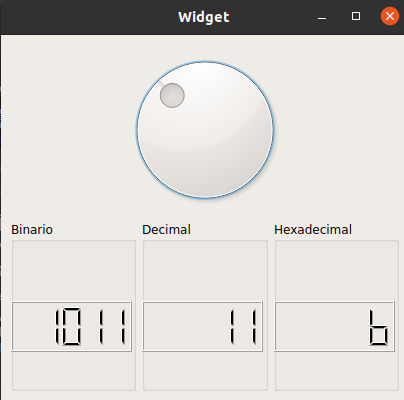
\includegraphics[scale=0.4]{images/DialNumber.png}
\end{figure}

El dial toma valores entre 0 y 31. Cuando este se mueve, los tres visores muestran el número asociado a la posición del dial en el formato respectivo.

\begin{questions}
	\question Utilizando el Qt Designer, agregue en su ventana principal 1 dial y 3 visores lcd. Puede utilizar layouts para mayor orden.
	\question Configure y conecte el dial con los visores lcd en cada formato. Utilice signals y slots para ello.	
\end{questions}
\newpage
\subsection*{Diales Hard mode}
Desarrolle el programa DialColor en C++ utilizando las bibliotecas Qt. Este programa cuenta con 3 diales y un cuadrado de dimensiones 50px por 50px y de color inicialmente negro dentro de una QGraphicsView. La disposición de los elementos así como los nombres de las variables asociadas a cada uno de estos se indican en la siguiente imagen:

\begin{figure}[H]
	\center
	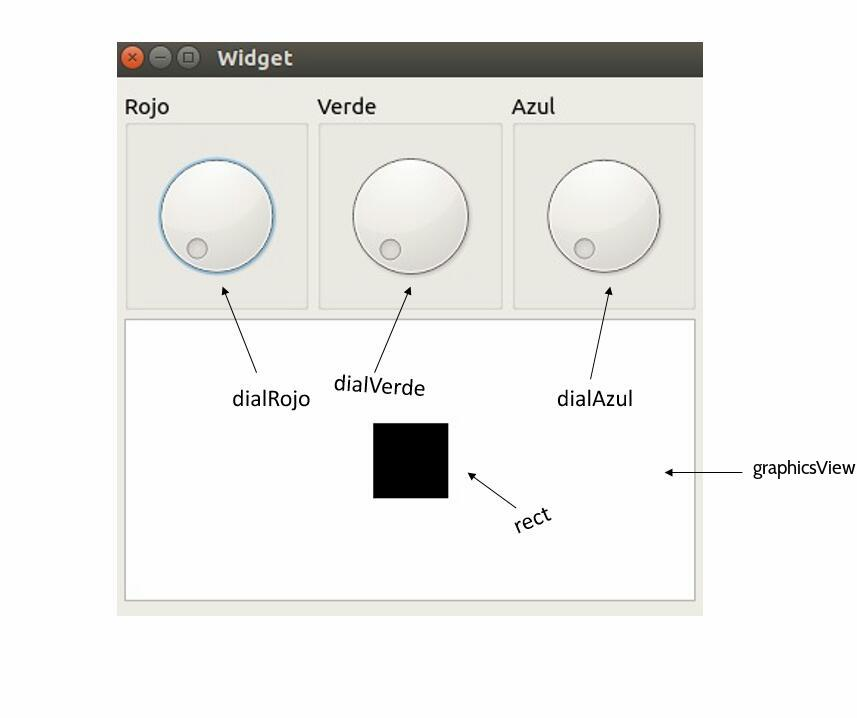
\includegraphics[scale=0.4]{images/DialColorUI.jpeg}
\end{figure}

Cada uno de los diales representa los colores rojo, verde y azul respectivamente y cuyos valores van del 0 al 255. El color del cuadrado viene dado por la combinación de los valores de la posición de cada uno de los diales en codificación RGB (Red-Green-Blue). Si uno de los diales se mueve, el color del cuadrado se actualiza con los nuevos valores presentes. 
En la página de Aula, se encuentra disponible el archivo \textbf{DialColor.zip}, el cual contiene el código base para el desarrollo del taller. 

\begin{questions}
	\question Estudie las clases QGraphicsView, QGraphicsScene y cómo estas se relacionan. 
	\question Estudie la clase QGraphicsRectItem y cómo asociarla a un objeto QGraphicsScene.
	\question Se ha creado la clase RectangleColor, la cual hereda de QGrapahicsRectItem para la visualización del cuadrado. Complete las implementaciones de los métodos \textbf{changeRed}, \textbf{changeGreen}, \textbf{changeBlue} y \textbf{updateColor} de la clase \textbf{RectangleColor}. Para el método \textbf{updateColor}, se recomienda utilizar las clases \textbf{QColor} y \textbf{QBrush}.
	\question En el constructor de la clase QWidget
	\begin{itemize}
		\item Cree el objeto QGraphicsScene scene y asócielo con la variable QGraphicsView graphicsView
		\item Cree el objeto cuadrado RectangleColor rect y añádala a la variable scene.
		\item Conecte cada uno de los QDial \textbf{dialRojo}, \textbf{dialVerde} y \textbf{dialAzul} a través de su signal \textbf{valueChanged} con el slot correspondiente de rect.
	\end{itemize}
\end{questions}

\end{document}
